\documentclass[a4paper, 12pt]{article}
\usepackage{titling}
\usepackage{array}
\usepackage{booktabs}
\usepackage{enumitem}
\usepackage{graphicx}
\usepackage{hyperref}
\usepackage{amssymb}
%\usepackage{mathtools}
\usepackage{listings}
\usepackage{amsmath}
\usepackage{color} %red, green, blue, yellow, cyan, magenta, black, white
\setlength{\heavyrulewidth}{1.5pt}
\setlength{\abovetopsep}{4pt}
\setlength{\parindent}{0pt}
\graphicspath{{.}}
\usepackage{float}
\usepackage[margin=1in]{geometry}
\definecolor{mygreen}{RGB}{28,172,0} % color values Red, Green, Blue
\definecolor{mylilas}{RGB}{170,55,241}
% Must be after geometry
\usepackage{fancyhdr}
\pagestyle{fancy}
\fancyhf{}
\rhead{NN Homework 7}
\lhead{P.Lukin, E. Ovchinnikova}
\cfoot{\thepage}

\setlength{\droptitle}{-5em}

\title{Neural Networks  \\
				- Homework 7 -}
\author{Petr Lukin, Evgeniya Ovchinnikova}
\date{Lecture date: 14 November 2016}

\begin{document}

%-------------------------------------------------------------------------------
\lstset{language=Matlab,%
    %basicstyle=\color{red},
    breaklines=true,%
    morekeywords={matlab2tikz},
    keywordstyle=\color{blue},%
    morekeywords=[2]{1}, keywordstyle=[2]{\color{black}},
    identifierstyle=\color{black},%
    stringstyle=\color{mylilas},
    commentstyle=\color{mygreen},%
    showstringspaces=false,%without this there will be a symbol in the places where there is a space
    numbers=left,%
    numberstyle={\tiny \color{black}},% size of the numbers
    numbersep=9pt, % this defines how far the numbers are from the text
    emph=[1]{break},emphstyle=[1]\color{red}, %some words to emphasise
    %emph=[2]{word1,word2}, emphstyle=[2]{style},
}

%-------------------------------------------------------------------------------

\maketitle

\section{Mind map}

\begin{figure}[h]
  \centering
  \caption{Mind map. Chapter 5 from Haykin's book. A zoomed version is attached as Radial-BasisFunctionNetworks.png}
  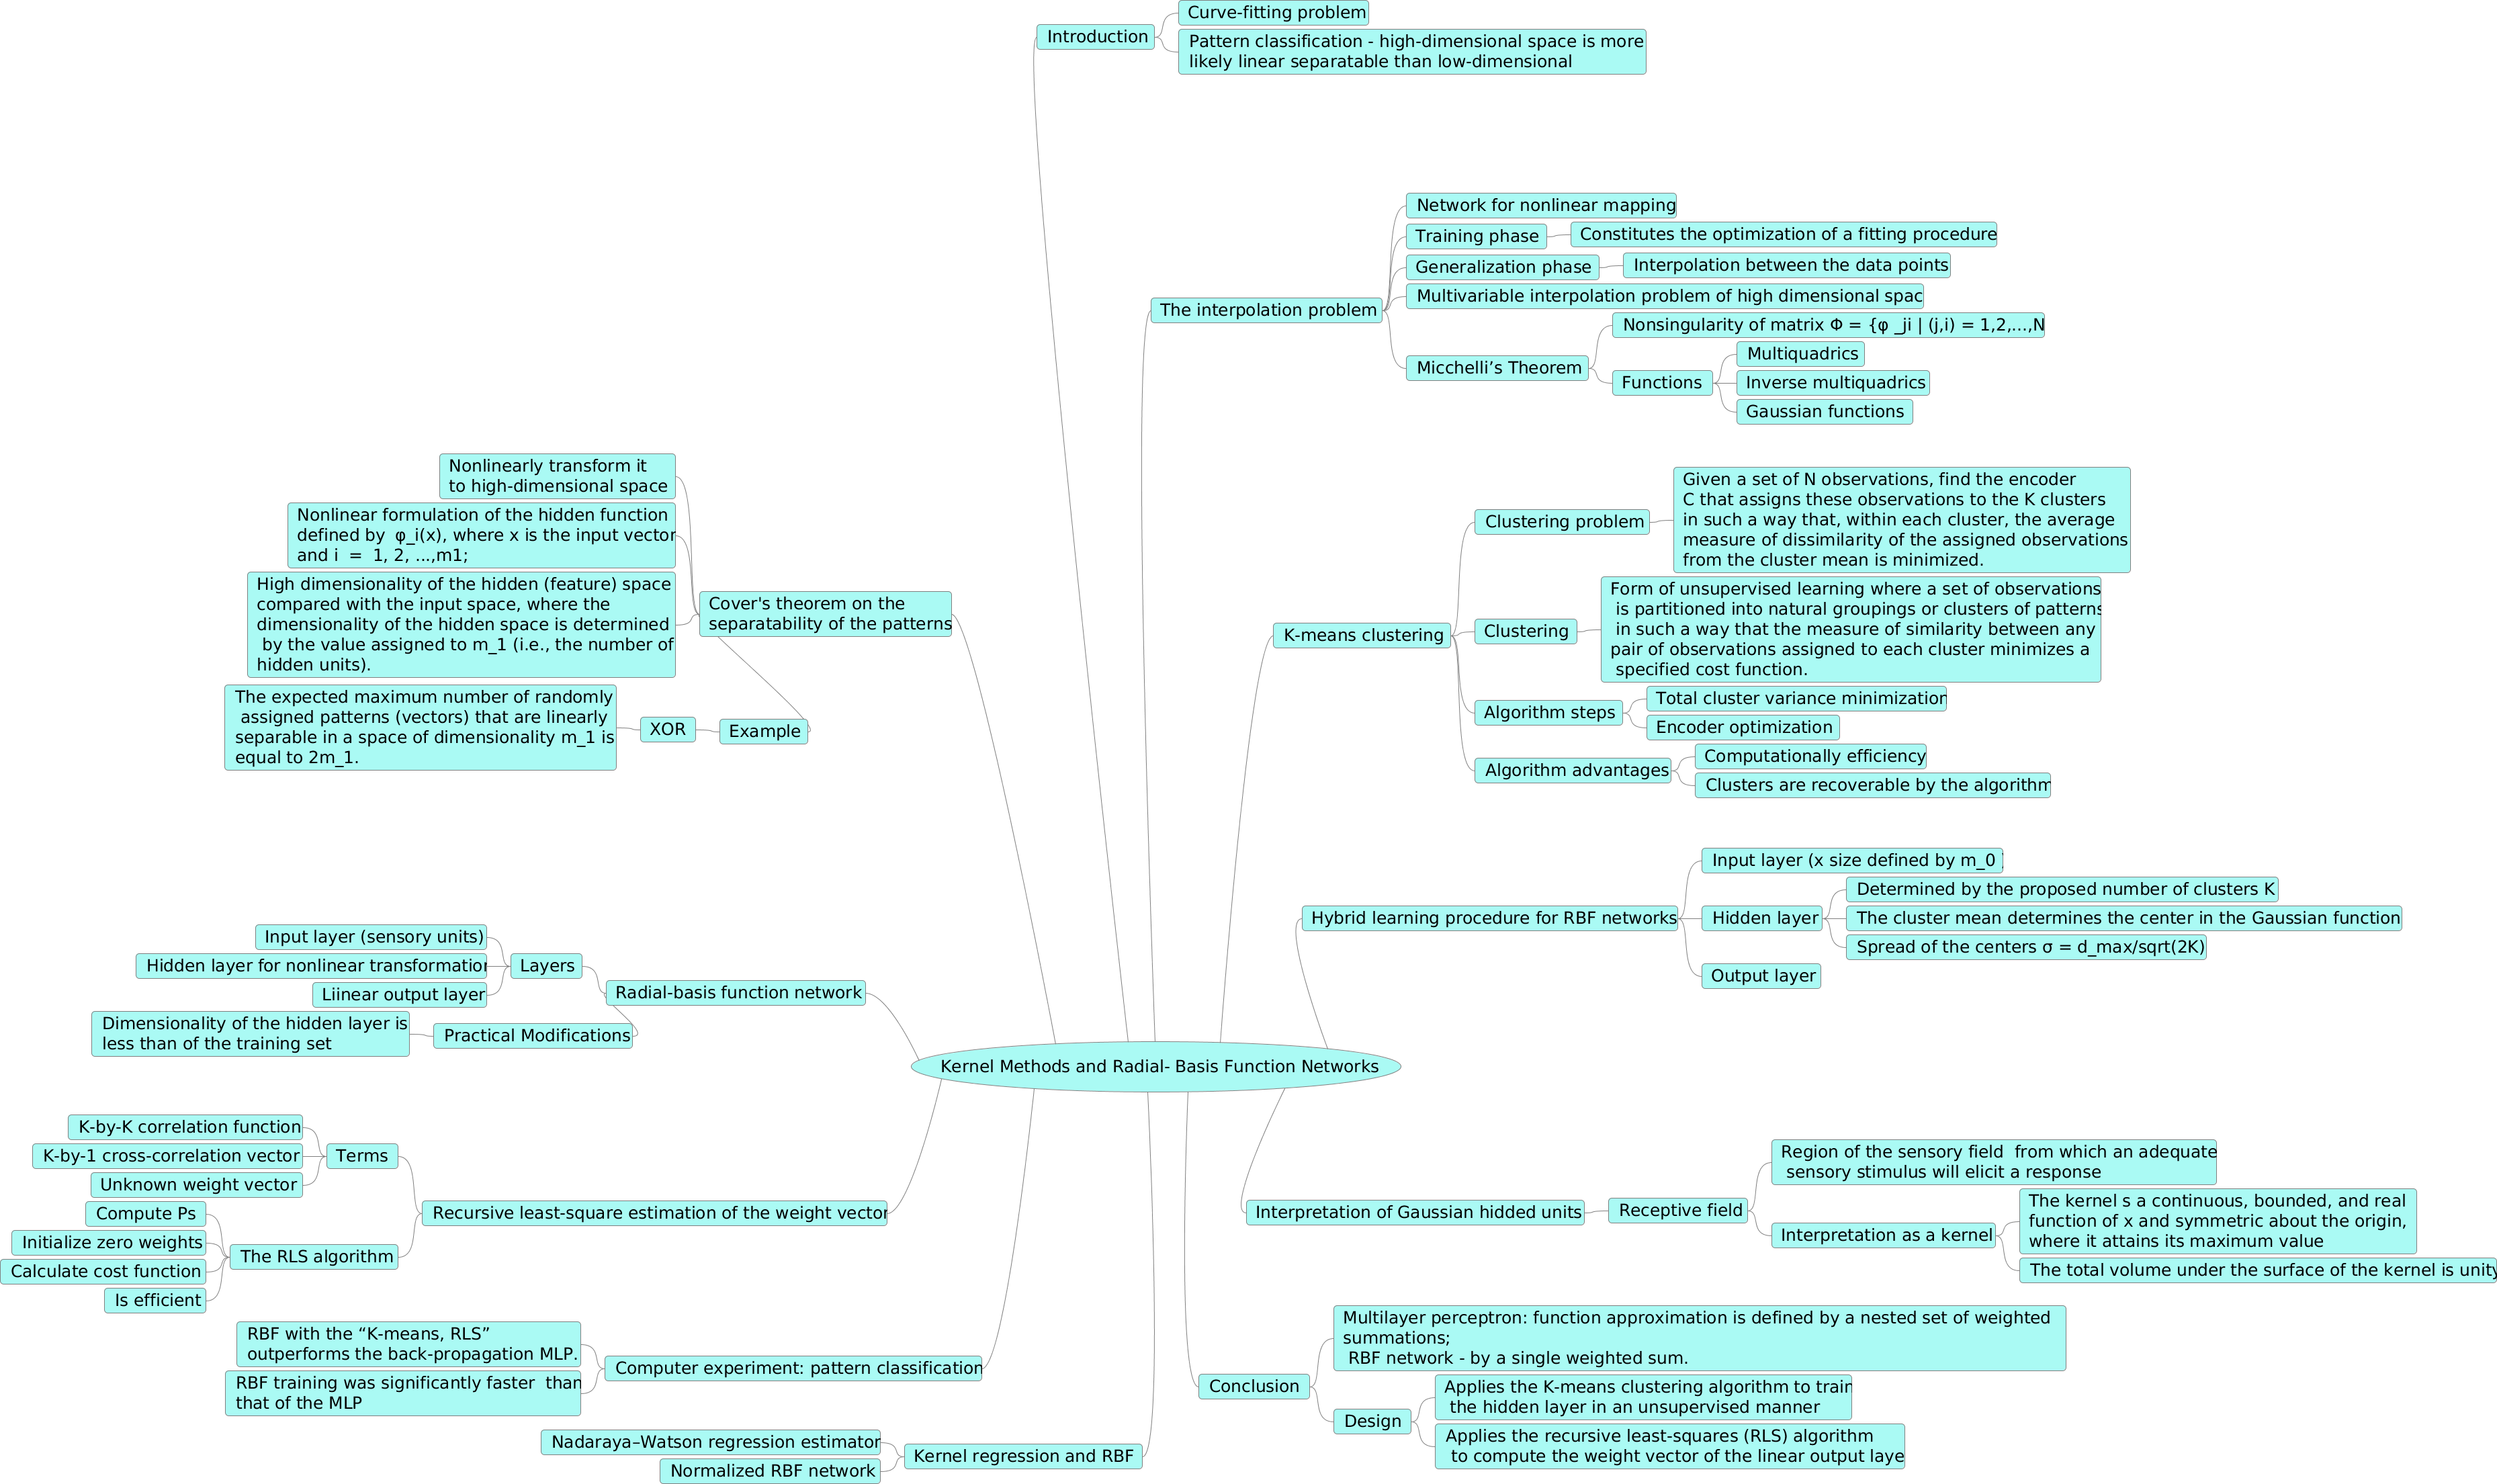
\includegraphics[width=1.0\textwidth]{Radial-BasisFunctionNetworks}
\end{figure}



\section{Exercises}

\subsection{Exercise 5.10}

The purpose of this computer experiment is to investigate the clustering process performed by the K-means algorithm. To provide insight into the experiment, we fix the number of clusters at K=6, but vary the vertical separation between the two moons in Fig. \ref{fig:moons}. Specifically, the requirement is to do the following, using an unlabled training sample of 1,000 data points picked randomly from the two regions of the double-moon pictured in Fig. \ref{fig:moons}:\\
\begin{itemize}
\item[(a)] Experimentally, determine the mean $\hat{\mu}_j$ and variance $\hat{\sigma}^2_j$, $j=1,2,..,6$, for the sequence of eight uniformly spaced vertical separations starting at $d=1$ and reducing them by one till separation $d=-6$ is reached.
\item[(b)] In light pf the results obtained in previous part, comment on how the mean $\hat{\mu}_j$ of cluster $j$ is affected by reducing the separation $d$ for $j=1,2$ and $3$.
\item[(c)] Plot the variance $\hat{\sigma}^2_j$ versus the separation $d$ for $j=1,2,...,6$.
\item[(d)] Compare the common $\sigma^2$ computed in accordance with the empirical formula of the equation $\sigma = \frac{d_{max}}{\sqrt{2K}}$ with the trends exhibited in the plots obtained in (c).
\end{itemize}

\begin{figure}[h]
  \centering
  \caption{The double moon classification problem \label{fig:moons}}
  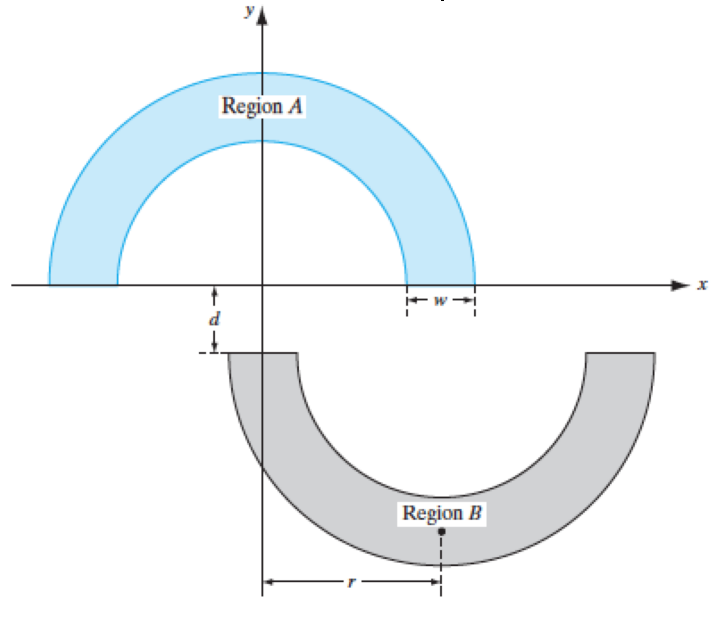
\includegraphics[width=0.5\textwidth]{moons}
\end{figure}

Solution:

\lstset{language=Python}
\begin{lstlisting}[frame=single]


\end{lstlisting}

\subsection{Exercise 5.11}
The purpose of this second experiment is to compare the classification performance of two hybrid learning algorithms: the "K-means,RLS" algorithm investigated in Section 5.8 and the "K-means,LMS" algorithm investigated in this problem.\\
	As in section 5.8, assume the following:\\
Number of hidden Gaussian units:20\\
Number of training samples:1,000 data points\\
Number of testing samples: 2,000 data points\\
Let the learning-rate parameter of the LMS algorithm be annealed linearly from 0.6 down to 0.01.
\begin{itemize}
\item[(a)] Construct the decision boundary computed for the "K-means,LMS" algorithm for the vertical separation between the two moons in Fig.\ref{fig:moons} set at $d=-5$.
\item[(b)] Repeat the experiment for $d=-6$.
\item[(c)] Compare the classification results obtained using the "K-means,LMS" algorithm with those of the "K-means,RLS" algorithm studied in Section 5.8.
\item[(d)] Discuss how, in general, the complexity of the "K-means,LMS" algorithm compares with that of the "K-means,RLS" algorithm.
\end{itemize}

\end{document}
